\section{静电场的分析}

\subsection{电势的定义}
根据\fancyref{ppt:静电场的旋度},电场强度$\vb*{E}$是无旋的
\begin{Equation}
    \curl\vb*{E}=\vb*{0}
\end{Equation}
根据\fancyref{def:无旋场的标势},无旋场可以定义标势,现在,我们定义$\vb*{E}$的标势。
\begin{BoxDefinition}[电势]
    定义电场强度$\vb*{E}$的标势为\uwave{电势}(Electric Potential),记作
    \begin{Equation}
        \vb*{E}(\vb*{r})=-\grad\varphi(\vb*{r})
    \end{Equation}
    这就是说,电势的负梯度是电场强度。
\end{BoxDefinition}

需要指出的是,由\fancyref{def:电势}给出的电势$\varphi$并不是唯一的,可以加上任意常数
\begin{Equation}
    \vb*{E}=-\grad\varphi=-\grad(\varphi+c)
\end{Equation}
而为了使得电场中每一点都具有一个确定的值,可以选定场中某一固定点为电势的参考点,即规定该参考点处的电势为零,这样任意常数$c$就可以被定出,从而使得电势可以被唯一确定。

\subsection{电势的计算}
\begin{BoxFormula}[电势]
    电势$\varphi(\vb*{r})$符合以下规律,以无穷远点为参考点
    \begin{Equation}
        \varphi(\vb*{r})=\frac{1}{4\pi\varepsilon}\Itnt[V]\frac{\rho(\vb*{r}')}{R}\dd{V'}
    \end{Equation}
\end{BoxFormula}
\begin{Proof}
    根据\fancyref{fml:电场强度}
    \begin{Equation}&[1]
        \vb*{E}(\vb*{r})=\frac{1}{4\pi\varepsilon_0}\Itnt[V]\frac{\rho(\vb*{r}')\vb*{R}}{R^3}\dd{V'}
    \end{Equation}
    现在我们考虑的是介质中的一般情况,故将$\varepsilon_0$替换为$\varepsilon$
    \begin{Equation}&[2]
        \vb*{E}(\vb*{r})=\frac{1}{4\pi\varepsilon}\Itnt[V]\frac{\rho(\vb*{r}')\vb*{R}}{R^3}\dd{V'}
    \end{Equation}
    根据\fancyref{fml:距离反比的梯度}
    \begin{Equation}&[3]
        \grad(\frac{1}{R})=-\frac{\vb*{R}}{R^3}
    \end{Equation}
    将\xrefpeq{3}代入\xrefpeq{2},并注意到$\grad$是可以提出积分外的
    \begin{Equation}&[4]
        \vb*{E}(\vb*{r})=\frac{1}{4\pi\varepsilon}\Itnt[V]-\grad(\frac{\rho(\vb*{r}')}{R})\dd{V'}=-\grad\qty(\frac{1}{4\pi\varepsilon}\Itnt[V]\frac{\rho(\vb*{r}')}{R}\dd{V'})
    \end{Equation}
    而根据\fancyref{def:电势}
    \begin{Equation}&[5]
        \vb*{E}(\vb*{r})=-\grad\varphi(\vb*{r})
    \end{Equation}
    比较\xrefpeq{4}和\xrefpeq{5},注意到电势有一个常数的任意性
    \begin{Equation}&[6]
        \varphi(\vb*{r})=\frac{1}{4\pi\varepsilon}\Itnt[V]\frac{\rho(\vb*{r}')}{R}\dd{V'}+c
    \end{Equation}
    假若我们取$c=0$
    \begin{Equation}&[7]
        \varphi(\vb*{r})=\frac{1}{4\pi\varepsilon}\Itnt[V]\frac{\rho(\vb*{r}')}{R}\dd{V'}
    \end{Equation}
    由于电荷均在有限远处,故\xrefpeq{7}的$\phi(r)$在无穷远处趋于零,即以无穷远为电势参考点。
\end{Proof}

在实践中,如果我们需要分析给定的电荷分布形成的电场,由于电场强度$\vb*{E}$是矢量,直接通过\fancyref{fml:电场强度}计算会比较繁琐,我们往往会先用\fancyref{fml:电势}先计算处标量电势$\varphi$的分布,随后再通过$\vb*{E}(\vb*{r})=-\grad\vb*{\varphi(\vb*{r})}$求出电场强度,以简化计算的复杂度。

\subsection{电势的物理意义}
\begin{BoxFormula}[电势的物理意义]
    电场强度和电势间具有以下关系
    \begin{Equation}
        \Int[P][Q]\vb*{E}(\vb*{r})\cdot\dd{\vb*{l}}=\varphi(P)-\varphi(Q)
    \end{Equation}
\end{BoxFormula}
\begin{Proof}
    实际上,这就是曲线积分基本定理的直接结果,不过我们还是来证明一下。

    根据\fancyref{def:电势}
    \begin{Equation}
        \vb*{E}(\vb*{r})=-\grad\varphi(\vb*{r})
    \end{Equation}
    在上式两端点乘$\dd{\vb*{l}}$,而梯度在某一方向的投影即该方向上的方向导数
    \begin{Equation}
        \vb*{E}(\vb*{r})\cdot\dd{\vb*{l}}=
        -\grad\varphi(\vb*{r})\cdot\dd{l}=-\pdv{\varphi}{l}\dd{\vb*{l}}=-\dd{\varphi(\vb*{r})}
    \end{Equation}
    积分即得
    \begin{Equation}*
        \Int[P][Q]\vb*{E}(\vb*{r})\cdot\dd{\vb*{l}}=\Int[P][Q]-\varphi(\vb*{r})=\varphi(P)-\varphi(Q)\qedhere
    \end{Equation}
\end{Proof}
\fancyref{fml:电势的物理意义}指出,在$P,Q$间的电势差$\varphi(P)-\varphi(Q)$的物理意义是\footnote{特别注意,当我们说$P,Q$两点间的电势差时,\textbf{是起点减去终点},即$\varphi(P)-\varphi(Q)$,而不是反之。}:将单位正电荷从点$P$沿任意路径移动到$Q$的过程中,电场力所做的功即$P,Q$间的电势差
\begin{itemize}
    \item 若电势差$\varphi(P)-\varphi(Q)$为正,则$P\to Q$的过程中电势减小,做功为正。
    \item 若电势差$\varphi(P)-\varphi(Q)$为负,则$P\to Q$的过程中电势增加,做功为负。
\end{itemize}

\subsection{电场的可视化}

通常,我们会用电场线和等势面形象描绘电场强度$\vb*{E}(\vb*{r})$和电势$\varphi(\vb*{r})$在空间的分布情况,而根据\fancyref{def:电势},电场线总是垂直于等势面,电场线指向的是电势下降最快的方向。\goodbreak

\xref{fig:电场线和等势面}中,我们分别绘制了等量异号点电荷和等量同号点电荷的电场线和等势面\footnote{这里仅绘制了点电荷所在平面上的电场,因此等势面表现为一条曲线。}
\begin{Figure}[电场线和等势面]
    \begin{FigureSub}[等量异号点电荷]
        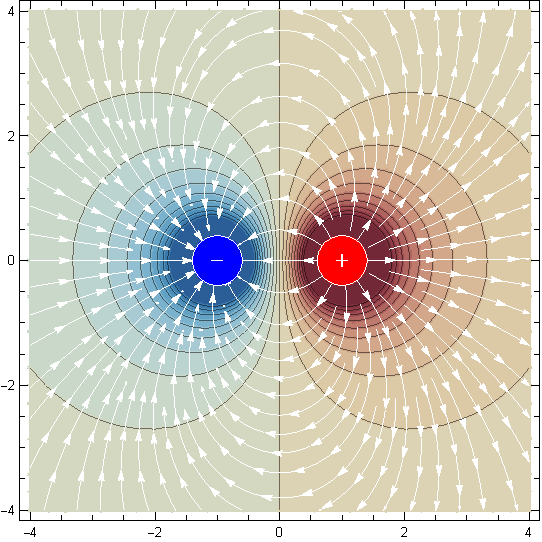
\includegraphics[width=6cm]{Mathematica/output/EFieldPN.pdf}
    \end{FigureSub}
    \hspace{1cm}
    \begin{FigureSub}[等量同号点电荷]
        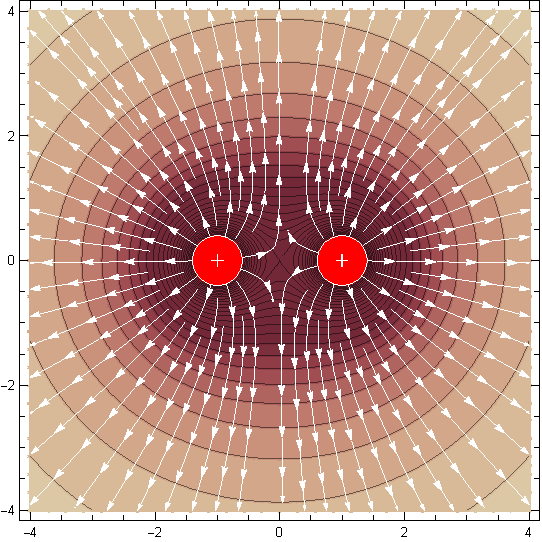
\includegraphics[width=6cm]{Mathematica/output/EFieldPP.pdf}
    \end{FigureSub}
\end{Figure}
\xref{fig:电场线和等势面}中的颜色意义如下:红色代表正电势,蓝色代表负电势。

\subsection{电势的微分方程}
在静电场中,我们往往会将电场的矢量方程及其边界条件
\begin{Gather}[6pt]
    \curl\vb*{E}=\vb*{0}\qquad
    \vb*{e}_\text{n}\times(\vb*{E}_1-\vb*{E}_2)=\vb*{0}\\
    \div\vb*{D}=\rho\qquad
    \vb*{e}_\text{n}\cdot(\vb*{D}_1-\vb*{D}_2)=\rho_S
\end{Gather}
转化为关于电势$\phi(\vb*{r})$的标量方程,因为矢量微分方程的求解要比标量微分方程复杂很多。

转化是怎么实现的呢?这就是本小节要达成的目标了。
\begin{BoxEquation}[静电场的微分方程]
    静电场可以由电势的泊松方程描述
    \begin{Equation}&[A]
        \laplacian\varphi=-\frac{\rho(\vb*{r})}{\varepsilon}
    \end{Equation}
    边界条件满足
    \begin{Equation}&[B]
        \varphi_1=\varphi_2\qquad
        \varepsilon_1\pdv{\varphi_1}{n}-\varepsilon_2\pdv{\varphi_2}{n}=-\rho_S
    \end{Equation}
\end{BoxEquation}

\begin{Proof}
    根据\fancyref{eqt:麦克斯韦方程组}和\fancyref{def:电势}
    \begin{Equation}&[1]
        \rho=\div\vb*{\vb*{D}}=\div(\varepsilon\vb*{E})=-\div(\varepsilon\grad\varphi)
    \end{Equation}
    我们知道,梯度的散度是拉普拉斯
    \begin{Equation}&[2]
        \rho=-\varepsilon\laplacian\varphi
    \end{Equation}
    移项即得\xrefpeq{A}
    \begin{Equation}&[3]
        \laplacian\varphi=-\frac{\rho}{\varepsilon}
    \end{Equation}
    下面我们来将$\vb*{E},\vb*{D}$的边界条件转化为$\varphi$的边界条件,如\xref{fig:电介质界面处的电位}所示,设$P_1$和$P_2$是位于不同电介质界面两侧紧贴分界面的相邻两点,记其电位分别为$\varphi_1$和$\varphi_2$,记其间距为$\delt{l}$。
    \begin{Figure}[电介质界面处的电位]
        \includegraphics{build/Chapter03A_01.fig.pdf}
    \end{Figure}

    正如我们在数学物理方法中学过的,由于$\varphi$满足的是二阶微分方程,故需要两个边界条件
    \begin{enumerate}
        \item 电位$\varphi$在边界两侧的关系(第一类边值条件)。
        \item 电位沿边界面法向的一阶方向导数$\pdv*{\phi}{n}$在边界两侧的关系(第二类边值条件)。
    \end{enumerate}
    由于$\vb*{E}$为有限值,当$P_1,P_2$的间距$\delt{l}\to 0$时,有
    \begin{Equation}&[4]
        \varphi_1-\varphi_2=\Lim[\delt{l}\to 0]\Int[P_1][P_2]\vb*{E}\cdot\dd{\vb*{l}}=\Lim[\delt{l}\to 0]\vb*{E}\cdot\dd{\vb*{l}}=0
    \end{Equation}
    因此,分界面两侧的电势是相等的
    \begin{Equation}&[5]
        \varphi_1=\varphi_2
    \end{Equation}
    而根据\fancyref{fml:电位移矢量的边界条件}
    \begin{Equation}&[6]
        \vb*{e}_\text{n}\cdot(\vb*{D}_1-\vb*{D}_2)=\rho_S
    \end{Equation}
    运用\fancyref{def:电势},在\xrefpeq{6}中代入$D=\varepsilon\vb*{E}=-\varepsilon\grad\phi$
    \begin{Equation}&[7]
        \vb*{e}_\text{n}\cdot(\varepsilon_1\grad\varphi_1-\varepsilon_2\grad\varphi_2)=-\rho_S
    \end{Equation}
    正如前面推导中提到过的,梯度在某个方向上的投影即为该方向上的方向导数
    \begin{Equation}&[8]
        \varepsilon_1\pdv{\varphi_1}{n}-\varepsilon_2\pdv{\varphi_2}{n}=-\rho_S
    \end{Equation}
    至此,我们就得到了所需的两个边界条件。
\end{Proof}